\documentclass{article}

\usepackage{geometry}
\usepackage[utf8]{inputenc}
\usepackage{amsmath}
\usepackage{wasysym}
\usepackage{amssymb}
\usepackage{hyperref}
\usepackage[ruled,vlined,linesnumbered]{algorithm2e}
\usepackage{listings}
\usepackage{graphicx}
\graphicspath{ {./pictures/} }
% \usepackage[style=numeric]{biblatex}
% \addbibresource{sources.bib}

\newcommand{\todo}{\paragraph{$\star$ TODO:}}
\newcommand{\sref}[1]{(section \ref{#1})}
\newcommand{\alp}{ArrayList$<$Point$>$}
\newcommand{\method}[4]{\underline{\textit{#1} #2 \textbf{#3}(#4)}}
\newcommand{\prop}[3]{\underline{\textit{#1} #2 \textbf{#3}}}
\DeclareMathOperator*{\argmin}{argmin}


\geometry{
  a4paper,
  total={170mm,257mm},
  left=25mm,
  top=25mm,
}

\title{Informatics Large Practical: Report}%\\\,\\Or\\Book 3: The Voyage of the Aftern$\infty$n Drone}
\author{Samo Nov\'ak\\(s1865783)}
\date{Semester 1, 2020/2021}

\begin{document}

\maketitle

\tableofcontents

\pagebreak

%%%%%%%%%%%%%%%%%%%%%%%%%%%%%%%%%%%%%%%%%%%%%%%%%%%%%%%%%%%%%%%%%%%%%%%%%%%%%%%%%%%%%%%%%%


\section{Software architecture description}

This section describes the architecture of the project in terms of classes and their interaction. The classes can be in general split into two categories: functional classes that perform computation and control the drone, and data classes which act as data storage.

\subsection{Functional classes}

The main class of the project is \textbf{AirQualityMapsApp} \sref{cls:AirQualityMapsApp}. This is used for running the program - it takes the inputs, instantiates other classes and calls the appropriate method. It is the ultimate controller of the program's execution.

The first class used by \textbf{AirQualityMapsApp} is the class \textbf{WebClient} \sref{cls:WebClient}. This performs all access to the web server and provides methods to load the different types of content needed. It was chosen to separate all of the workings of the web interface from the rest of the program.

The computations for the drone itself are split between different phases:
\begin{itemize}
\item \textit{planning} -- this constitutes creating a high-level sequence of waypoints as guidance for the drone, which is an abstract representation of the drone's objectives,
\item \textit{control/simulation} -- during which the drone takes the high-level flight plan an executes it, taking into account contraints on its motion created by the specification (individual steps are of length $0.0003$ degrees; allowed directions are multiples of $10$ degrees, counterclockwise from the axis of positive longitude), as well as the no-fly zones and the boundaries of the confinement area. In the future development, this could also include corrections for wind and other environemntal influences.
\end{itemize}

The planning phase is performed by the \textbf{PathPlanner} class \sref{cls:PathPlanner}, which creates a sequence of waypoints, taking into account the locations of sensors and their distance from each other, as well as the obstacles, i.e. no-fly zones defined around certain buildings.

The \textbf{PathPlanner} works together with the \textbf{ObstacleEvader} class \sref{cls:ObstacleEvader}, which provides support for geometrical computation: it helps with finding intersections of possible plan segments with the no-fly zones. This also takes care of the confinement area, which is seen as a no-fly zone extending outwards from the boundaries.

The other phase, control (and so far simulation, as this project merely simulates a possible future drone), is embodied by the class \textbf{DroneController} \sref{cls:DroneController}. This class is responsible for controlling the flight of the drone, following the waypoints generated by \textbf{PathPlanner}. It interacts with the \textbf{ObstacleEvader} as well, making sure each step is valid, i.e. does not intersect a no-fly zone, and by extension that it does not cross the boundaries of the confinement.

\subsection{Data classes}

These classes serve as storage and processing of data. In particular, classes \textbf{W3WDetails} and \textbf{SensorReading} are used for deserializing JSON data from the web server, which is a requirement of the library \textit{GSON} used to process JSON files.

\textbf{W3WDetails} \sref{cls:W3WDetails} holds the translation of a \textit{What 3 Words} address into a location in terms of longitude and latitude.

The sensor locations, along with their readings (for the purpose of this project, which simulates the sensors) are held in \textbf{SensorReading} \sref{cls:SensorReading}.

Each no-fly zone, including the space outside of confinement, is represented as a polygon describing its external boundary (i.e. there are no holes in the zones - these would be unreachable anyway). This is ultimately encoded as a list of points. However, since these are very common in the code, in order to improve readability and make intentions clear, a new class \textbf{Obstacle} \sref{cls:Obstacle}, which contains those points, is used to represent the no-fly zones. 

There is a class \textbf{Move} \sref{cls:Move}, which represents a move that the drone can make. It is beneficial to have all the data about a move in one place, because it simplifies the storage of data and its serialization into output files.

Another abstraction, in this case an \textit{enum}, is \textbf{RotationDirection} \sref{cls:RotationDirection}, which encodes the direction of rotation (in the usual sense of positive being counterclockwise, with axis taken to go upwards). This would be easily encoded with just numbers, but the enum abstraction makes the usage more clear in terms of semantics, and also limits the allowed values. 

The class \textbf{ColoursSymbols} \sref{cls:ColoursSymbols} is responsible for generating properties of markers -- their colour and symbol -- based on the data read from sensors. Similarly to previous classes, it is used to that everything that has to do with colours and symbols of markers is in one place.

\subsubsection{Miscellaneous}

The code base contains two more classes. These are separate in a way -- though they are used to handle data, they are used more as a convenience.

The first of these is class \textbf{Pair$<$Left, Right$>$} \sref{cls:Pair}, where \textbf{Left} and \textbf{Right} are arbitrary types. This represents an arbitrary pair ($2$-tuple) of possibly different data types, and is designed to mimic the behaviour of languages where creation of arbitrary tuples is commonplace. I use it to return multiple values from a single function call, where the two values are related (belong together in some way) and it would be inconvenient to create a new class for this purpose.

The other class in this section relates to \textbf{WebClient} and it is the \textbf{WebClientException} \sref{cls:WebClientException}, which unifies all the reasonably expectable exceptions from the \textbf{WebClient}. The reason for using such class is that, while there are many possible things that can go wrong when trying to load data from a web server, these should all be ultimately handled the same way: the program should terminate, because it is impossible to do anything of value without having the data from the server. Therefore, this single unified exception is provided, so that the program knows that an error happened in the web server.

\subsection{External libraries}

The project includes two external libraries: \textbf{GSON}, Google's libary for processing JSON in general, and \textbf{GeoJSON}, MapBox's library for handling GeoJSON (JSON containing geographical data) in particular.


\section{Class documentation}
\label{class-documentation}

\subsection{AirQualityMapsApp}
\label{cls:AirQualityMapsApp}

The main class of the project. It has the following methods:

\subsubsection*{Methods}

\begin{itemize}
\item \method{public static}{void}{main}{String[\,] args} \\
  The main function of the program. Handles the terminal arguments which are: day, month, year, latitude, longitude, randomness seed (not used in the program), server port. This is the part of the codebase which controls all the rest.
\item \method{private static}{String}{formatDateDMY}{int day, int month, int year} \\
  A helper function used to format the date as \verb|DD-MM-YYYY|.
\end{itemize}


\subsection{WebClient}
\label{cls:WebClient}

Web client used for loading (and parsing) relevant data from the HTTP server. It contains the following local properties and methods:

\subsubsection*{Properties}

\begin{itemize}
\item \prop{private final}{String}{host} \verb|= "http://localhost";| \\
  The connection host. It has the value \textit{localhost}, as the program is connecting to a local server.
\item \prop{private final}{int}{port} \\
  Web server port.
\item \prop{private}{HttpClient}{client} \\
  The client instance. Instantiated once with and then used throughout.
\end{itemize}

\subsubsection*{Methods}

\begin{itemize}
\item \underline{\textit{public} \textbf{WebClient}(int port)} -- constructor
  
\item \method{private}{String}{load}{String path} \\
  The internal method for loading data as a \textbf{String} from the server. \\
  On error, it throws \textbf{WebClientException} \sref{cls:WebClientException}.
\item \method{public}{ArrayList$<$SensorReading$>$}{loadSensorList}{int year, int month, int day} \\
  Load and parse the list of sensors for a particular day, which is returned as a list of \textbf{SensorReading} \sref{cls:SensorReading}. Uses the next function to translate \textit{What 3 Words} addresses.\\
  Also throws \textbf{WebClientException}.
  
\item \method{private}{Point}{loadPointFromWords}{String words} \\
  Translate an address in \textit{What 3 Words} into a \textbf{Point} (a class from \textit{MapBox GeoJSON} library).\\
  Throws \textbf{WebClientException}.

\item \method{public}{FeatureCollection}{loadNoFlyZones}{} \\
  Loads no-fly zones, parses them using \textit{MapBox GeoJSON}. \\
  Throws \textbf{WebClientException}.
\end{itemize}


\subsection{PathPlanner}
\label{cls:PathPlanner}

The class responsible for high-level planning of waypoints for the drone to follow.

\subsubsection*{Properties}

\begin{itemize}
\item \prop{private final}{ArrayList$<$SensorReading$>$}{sensorList} \\
  Contains the list of sensors as \textbf{SensorReading}.
\item \prop{private final}{int}{NUMBER\_OF\_SENSORS} \\
  The number of sensors. This is used in the path-finding and optimization methods of the Planner.
\item \prop{private}{double[\,][\,]}{distances} \\
  The distance matrix of the undirected weighted graph containing as vertices the locations of sensors and also the initial drone location.\\
  Has the property that $\mathrm{distances}[i][j] \equiv \mathrm{distances}[j][i]\,\forall i,j$ (i.e. is \textit{symmetric}). (See section \ref{alg:intro})
\end{itemize}

\subsubsection*{Methods}

\begin{itemize}
\item \underline{\textit{public} \textbf{PathPlanner}(ObstacleEvader evader, ArrayList$<$SensorReading$>$ sensorList)} -- constructor \\
  Apart from storing values, it also precalculates the distance matrix for later use.
\item \method{private}{double}{distance}{Point x, Point y} \\
  Computes the Euclidean distance between the two points.
\item \method{public}{\alp}{findPath}{double startLatitude, double startLongitude} \\
  The function for finding waypoints to guide the drone. Calculates the distance matrix entries for the drone initial position, and generates the sequence of waypoints using \textbf{solveTSP} (see below).
\item \method{private}{\alp}{solveTSP}{} \\
  Generates the sequence of sensors to be visited in an order that is heuristically efficient. It works by recasting the problem as a \textit{Travelling Salesperson Problem} (TSP), where the vertices of the graph are sensor locations. The initial TSP circuit is generated by \textbf{nearestInsert} and then optimized by \textbf{flipSwap} (see both below).
  It \textbf{guarantees} that the drone's initial location is the first element of the 
sequence.

\item \method{private}{\alp}{nearestInsert}{} \\
  Generates a TSP circuit using the \textit{Nearest Insert} heuristic. (See Algorithm \ref{alg:nearest-insert})

\item \method{private}{void}{flipSwap}{\alp \,\,sequence} \\
  Optimize (in place) the given TSP circuit (sequence of vertices) using the \textit{Flip + Swap} heuristic. (See Algorithm \ref{alg:flip-swap})
\end{itemize}


\subsection{ObstacleEvader}
\label{cls:ObstacleEvader}

This class is used to handle the geometry of obstacles (the no-fly zones) - finding whether lines (e.g. flight path segments or drone moves) intersect any of them; and to help the drone with their evasion.

\subsubsection*{Properties}

\begin{itemize}
\item \prop{private final}{double}{LAT\_MAX, LAT\_MIN, LON\_MAX, LON\_MIN} \\
  Boundaries of the confinement area.
\item \prop{private}{ArrayList$<$Obstacle$>$}{noFlyZones} \\
  Array containing no-fly zones as lists of Points
\item \prop{private}{HashMap$<$Obstacle, Point$>$}{averages} \\
  A hash map assigning to each no-fly zone the average of its points, meant to be the zone's centre in a way.
\end{itemize}

\subsubsection*{Methods}

\begin{itemize}
\item \underline{\textit{public} \textbf{ObstacleEvader}(FeatureCollection noFlyZones)} -- constructor \\
  During initiation, it also unpacks the no-fly zones from a list of \textbf{Feature} to a list of \textbf{Obstacle}s. It adds the confinement area to this list as well, as all space outside the confinement can be seen as another no-fly zone. For each zone, it computes the centre (see \textbf{averages} above).
\item \method{private}{Point}{getAveragePoint}{List$<$Point$>$ points} \\
  Compute the average point. Does not count the last point into this average, because that is always the same as the first (due to the points coming from a closed polygons).
\item \method{public}{boolean}{crossesAnyObstacles}{Point a1, Point a2} \\
  Checks if any of the no-fly zones are crossed by a line segment from a1 to a2 (denoted a1 --- a2).
\item \method{public}{Obstacle}{nearestCrossedObstacle}{Point a1, Point a2} \\
  Find the obstacle intersected by the line segment a1 --- a2. If multiple obstacles are found, returns the one that is nearest to a1.
\item \method{private}{ArrayList$<$Obstacle$>$}{allCrossedObstacles}{Point a1, Point a2} \\
  Finds all the zones crossed by this line.
\item \method{private}{boolean}{crossesOneObstacle}{Point a1, Point a2, Obstacle obstacle} \\
  Checks if the line segment a1 --- a2 crosses the obstacle.
\item \method{private}{ArrayList$<$Pair$<$Point, Integer$>>$}{obstacleIntersections}{Point a1, Point a2, Obstacle obstacle} \\
  Finds all the intersections of line segment a1 --- a2 with the obstacle. It returns a list of \textbf{Pair}s, where \textit{left} is the point of intersection and \textit{right} is the index $i$ of the vertex of the polygon, such that a1 --- a2 intersects the line segment $i$ --- $((i + 1) \mod n)$, where $i, (i+1)\mod n$ are points at respective indices of the obstacle and $n$ is the number of points of the obstacle.
\item \method{private}{Point}{intersection}{Point a1, Point a2, Point b1, Point b2} \\
  Finds the point of intersection of the lines a1 --- a2 and b1 --- b2.
\item \method{public}{RotationDirection}{chooseEvasionDirection}{Obstacle obstacle, Point origin, double angle} \\
  Decide in which direction the drone should go to avoid this obstacle. (See \ref{alg:evasion})
\end{itemize}


\subsection{DroneController}
\label{cls:DroneController}

The class responsible for controlling (simulating) the drone operations, collecting data from sensors and exporting data into the output files.

\subsubsection*{Properties}

\begin{itemize}
\item \prop{private final}{double}{MOVE\_LENGTH} = $0.0003$ \\
  Length of allowed drone moves.
\item \prop{private final}{double}{SENSOR\_READ\_MAX\_DISTANCE} = $0.0002$ \\
  Maximum distance over which the drone is able to connect to a sensor. It is not inclusive, meaning the actual distance has to be strictly less.
\item \prop{private final}{int}{MAX\_BATTERY} = $150$ \\
  Maximum (and initial) battery charge.
\\
\item \prop{private final}{ArrayList$<$SensorReading$>$}{sensors, visitedSensors} \\
  List of all sensors on the map. (For \textbf{SensorReading} see \ref{cls:SensorReading})
\item \prop{private}{ArrayList$<$SensorReading$>$}{visitedSensors} \\
  Those sensors that have already been visited.
\item \prop{private}{int}{battery} and \prop{private}{double}{latitude, longitude} \\
  The state variables of the drone. Battery is initialized to \textbf{MAX\_BATTERY}.
\item \prop{private}{ArrayList$<$Move$>$}{trajectory} \\
  The record of all the moved made by drone. (for \textbf{Move} see \ref{cls:Move})
\item \prop{private}{ObstacleEvader}{evader} \\
  Used for avoiding hitting no-fly zones.
\end{itemize}

\subsubsection*{Methods}

\begin{itemize}
\item \underline{\textit{public} \textbf{DroneController}(ArrayList$<$SensorReading$>$ sensors, ObstacleEvader evader)} -- constructor
\item \method{public}{void}{executePathPlan}{\alp\,\,waypoints} \\
  Takes the high-level waypoints and navigate the drone along them, updating its internal state at every point and recording moves in \textbf{trajectory}. (See \ref{alg:drone-control})
  
\item \method{private}{Point}{computeMove}{double angle} \\
  Return the location where the drone would arrive after executing a move in specified angle from its current location.

\item \method{private}{Obstacle}{moveIntersectsObstacle}{Point end} \\
  Return the nearest no-fly zone intersected by a move from the current location to end.
  
\item \method{private}{ArrayList$<$SensorReading$>$}{getUnvisitedSensorsInRange}{} \\
  Gets the sensors that are in the drone's current range, could be read and have not been read yet.

\item \method{private}{double}{droneDistance}{SensorReading sensor \textit{OR} Point pt} \\
  Computes the distance to the sensor or point from the current location of the drone.

\item \method{public}{void}{serializeTrajectory}{String flightpathFilename, String readingsMapFilename} \\
  Generates the flight-path and map files with specified filenames.

\item \method{private}{Feature}{createSensorMarker}{SensorReading sensor, boolean visited} \\
  Creates the marker for the specified sensor, taking into account whether thedrone was visited. This function uses \textbf{ColoursSymbols} \sref{cls:ColoursSymbols}.
\end{itemize}

\subsection{W3WDetails}
\label{cls:W3WDetails}

Class used to deserialize \textit{What 3 Words} address translations. It has no methods.

\subsubsection*{Properties}

\begin{itemize}
\item \underline{String \textbf{words}} -- the \textit{What 3 Words} address
\item \underline{CoordinatesObject \textbf{coordinates}} -- the coordinates \\
  \textbf{CoordinatesObject} is a local class that contains two doubles: \textbf{lng} (longitude) and \textbf{lat} (latitude). This is to reflect the format given in the files from web server.
\end{itemize}


\subsection{SensorReading}
\label{cls:SensorReading}

This class represents a sensor and its readings. It is used to deserialize sensor data from JSON.

\subsubsection*{Properties}

\begin{itemize}
\item \underline{String \textbf{location}} and \underline{double \textbf{lat}, \textbf{lon}} \\
  Location as \textit{What 3 Words} and also GPS.
\item \underline{double \textbf{battery}} and \underline{String \textbf{reading}} \\
  Data from the sensor - its battery and reading of air pollution.
\end{itemize}

\subsubsection*{Methods}

\begin{itemize}
\item \method{public}{Point}{toPoint}{} -- convert to \textit{MapBox GeoJSON} Point
\end{itemize}

\subsection{Obstacle}
\label{cls:Obstacle}

This class represents a no-fly zone, which is encoded as a list of points defining the zone's external boundaries. The class \textbf{Obstacle} is therefore a \textbf{subclass of}, and acts as an alias for: \textbf{ArrayList$<$Point$>$} (where \textbf{Point} is provided by \textit{MapBox GeoJSON} library). Functionally, it behaves the same, but I chose to use it to improve readability. Apart from having all the properties and methods of \textbf{ArrayList$<$Point$>$}, it also has:

\subsubsection*{Methods}

\begin{itemize}
\item \method{public static}{Obstacle}{fromList}{List$<$Point$>$ list} \\
  This is a static function that creates an instance of \textbf{Obstacle} from any kind of list containing points. It is needed when extracting a list of points from \textit{MapBox}'s class \textbf{Polygon}.
\end{itemize}

\subsection{Move}
\label{cls:Move}

This class is a representation of the drone's move. It is used to record trajectory and collected data.

\subsubsection*{Properties}

\begin{itemize}
\item \prop{private final}{Point}{original, next} \\
  Start and end point of the drone's step.
\item \prop{private final}{int}{direction} \\
  Direction in degrees.
\item \prop{private final}{SensorReading}{sensor} \\
  The recorded sensor readings at the end of the move.
\end{itemize}

\subsubsection*{Methods}

\begin{itemize}
\item \underline{\textit{public} \textbf{Move}(Point original, int direction, Point next, SensorReading sensor)} -- constructor
\item getters for \textbf{direction}, \textbf{sensor}, \textbf{original}, \textbf{next}
\item \method{public}{String}{serialize}{int moveNumber} \\
  This function serializes the \textbf{Move} in the format required by the specification for the \textit{flightpath} file. Argument moveNumber is the number of the move, i.e. the first part of the serialized string, and it is there because the \textbf{Move} does not know when it happened.
\end{itemize}

\subsection{RotationDirection}
\label{cls:RotationDirection}

An enumerated type that represents a direction of rotation. The convention used is the usual one, where positive rotation means going counterclockwise about some axis. This enum provides a nice semantic abstraction, in contrary to using just an integer value.

\subsubsection*{Values}

\begin{itemize}
\item \textit{None} -- corresponds to no rotation and is encoded by $0$
\item \textit{Positive} -- positive rotation (counterclockwise), encoded by $+1$
\item \textit{Negative} -- negative rotation (clockwise), encoded by $-1$
\end{itemize}

\subsubsection*{Properties}

\begin{itemize}
\item \prop{private}{int}{value} \\
  The internal storage of the value, which can be one of the above
\end{itemize}

\subsubsection*{Methods}

\begin{itemize}
\item \underline{\textbf{RotationDirection}(int value)} -- constructor
\item \method{public}{int}{getValue}{} \\
  Getter for \textbf{value}
\item \method{public}{boolean}{equal}{RotationDirection direction} \\
  Checks two objects of type \textbf{RotationDirection} for equality.
\end{itemize}

\subsection{ColourSymbols}
\label{cls:ColoursSymbols}

This is a class used to decide the properties of sensor markers. It contains two enums, implemented this way them because they provide a nice abstraction of the relevant values.

\begin{itemize}
\item \prop{public}{enum}{Colour} \\
  Values: \textit{Green, MediumGreen, LightGreen, LimeGreen, Gold, Oragne, RedOrange, Red, Black, Gray}
\item \prop{public}{enum}{Symbol} \\
  Values: \textit{Lighthouse, Danger, Cross, None}
\end{itemize}

Each enum has a property \prop{private}{String}{value}, that stores internally the string that the enumerated value corresponds to: in the case of \textbf{Colour} these are the hexadecimal colour codes; and in the case of \textbf{Symbol} these are symbol names. Each enum also has the following functions:

\subsubsection*{Methods of Colour and Symbol enums}

\begin{itemize}
\item \underline{\textbf{Colour}(String colour)} and \underline{\textbf{Symbol}(String symbolString)} -- constructors
\item \method{public static}{\{Colour \textit{OR} Symbol\}}{getFromPollution}{double pollution} \\
  Choose the appropriate enumerated value depending on the value of pollution. These functions assume a valid pollution value, i.e. $0\le$ pollution $<256$.
\item \method{public}{String}{getValue}{} -- getter for \textbf{value}
\end{itemize}

\subsubsection*{Methods of ColourSymbols}

\begin{itemize}
\item \method{public static}{Pair$<$Colour, Symbol$>$}{getColourSymbol}{String reading, double battery} \\
  Decides both the \textbf{Colour} and \textbf{Symbol} based on sensor readings. (For \textbf{Pair$<$Left, Right$>$} see \ref{cls:Pair}).
\item \method{public static}{Pair$<$Colour, Symbol$>$}{getNotVisited}{} \\
  Returns the properties of an unvisited sensor. To make it less expensive, it only returns a preexisting property \prop{private final static}{Pair$<$Colour, Symbol$>$}{notVisited}.
\end{itemize}


\subsection{Pair$<$Left, Right$>$}
\label{cls:Pair}

A generic class representing a pair (2-tuple) of arbitrary values and possibly different types. It mimicks the behaviour of 2-tuples in languages where they are prevalent - it is an immutable data type intended simply as storage. This construct is quite convenient for example when a function needs to return two related values of different types.

\subsubsection*{Properties}

\begin{itemize}
\item \prop{public final}{Left}{left}
\item \prop{public final}{Right}{right}
\end{itemize}

It is worth noting that both of these are constants and are directly accessible without the need of a getter function -- this is a deliberate due to \textbf{Pair} being a purely storage data type.

\subsubsection*{Methods}

\begin{itemize}
\item \underline{\textit{public} \textbf{Pair}(Left left, Right right)} -- constructor
\item \method{public}{Pair$<$Left, Right$>$}{clone}{} \\
  Function that returns a shallow clone of the original \textbf{Pair}. This means it creates a new \textbf{Pair} instance and assigns \textbf{left} and \textbf{right} to it respectively -- however it does not clone the internal values.
\end{itemize}


\subsection{WebClientException}
\label{cls:WebClientException}

This is a unifying exception class for multiple different exceptions that can occur when attempting to connect to the web server and load files from there. It is thrown by \textbf{WebClient} \sref{cls:WebClient}.

\subsubsection*{Properties}

\begin{itemize}
\item \prop{private static final}{long}{serialVersionUID} \\
  Serial number required by Java. No specific significance for our project.
\item \prop{private final}{String}{comment} \\
  Error message or comment.
\item \prop{private final}{Exception}{originalException} \\
  Used to store the original exception that caused the \textbf{WebClient} to thrown \textbf{WebClientException}. This is used for printing stack stace.
\end{itemize}

Both \textbf{comment} and \textbf{originalException} properties can be \textit{null}, but then the exception conveys little useful information. Conventionally, \textbf{comment} should not be \textit{null}.

\subsubsection*{Methods}

\begin{itemize}
\item \underline{\textit{public} \textbf{WebClientException}(String comment, Exception originalException)} -- constructor
\item \method{public}{void}{printStackTrace}{} \\
  This function prints the \textbf{comment} followed by the original stack trace that caused the exception (so the stack trace of \textbf{originalException}) if they exist. The values are printed to standard error output.
\end{itemize}

\section{Drone control algorithm}
\label{drone-algorithm}

As noted at the start, there are two phases of the drone control:
\begin{itemize}
\item \textit{planning} (handled by \textbf{PathPlanner} \sref{cls:PathPlanner})-- creating a high-level sequence of waypoints that the drone will later use for navigation, and
\item \textit{control/simulation} (handled by \textbf{DroneController} \sref{cls:DroneController}) -- executing this high-level plan, taking into account specific contraints on the drone's motion, such as no-fly zones.
\end{itemize}

This allows for efficient planning of overall order of sensors to visit, where the specific actions of the drone will be determined during the flight. This is beneficial also for the future development, when the drone might need to take into account wind and possibly other phenomena.

Both of these phases are are described in the following sections:

\subsection{Path planning}
\label{alg:intro}

In this first phase, the problem of navigation at hand can be reduced to an instance of the \textit{Travelling Salesperson Problem}. First, some definitions:

We have a \textit{complete undirected graph} $G=(V,E)$, where $V$ is the set of vertices and $E = V \times V$ is the set of edges, $N = |V|$ being the number of vertices. There is a weight function $w: E \to \mathbb{R}_{\ge 0}$ which assigns to each edge a real, nonzero weight; and which is symmetric, i.e. $\forall (u, v) \in E\ldotp\, w(u,v) = w(v,u)$.

The set $V$ of vertices contains the sensors (mainly the points where they are located) and the location where the drone starts. In the program, these vertices are represented as integers, such that a vertex $i \in V$ corresponds to the following
\begin{itemize}
\item the sensor at index $i$ in \textbf{PathPlanner.sensorList} if $i < N - 1$; where indexing starts at $0$,
\item the starting location of the drone if $i = N - 1$ (which is the maximum $i$).
\end{itemize}

The graph is complete (meaning all edges exist, $E = V \times V$), because the drone can conceivably travel between any two vertices.

The weight function is represented by the distance matrix \textbf{PathPlanner.distances} (which will be also denoted by $\mathbf{D}$, with components denoted $\mathbf{D}[i,j]$ for good readability). This weight function/distance matrix satisfies the following properties $\forall i,j \in V$:
\begin{align*}
  w(i,j)=\mathbf{D}[i,j]=\mathrm{\mathbf{PathPlanner.distances}}[i][j] \ge 0 && \mathbf{D}[i,j] = \mathbf{D}[j,i] && \mathbf{D}[i,i] = 0
\end{align*}

The components of $\mathbf{D}$ are not just defined by the Euclidean distance, however. Here, the \textbf{ObstacleEvader} \sref{cls:ObstacleEvader} comes into play and the distance matrix will depend on whether the particular edge intersects a no-fly zone:
\[
  \forall i\ne j \ldotp\, \mathbf{D}[i,j] =
  \begin{cases}
    \mathrm{EuclideanDistance}(i,j) & \mathrm{line\,between}\,i,j\,\mathrm{does\,not\,intersect\,obstacles} \\
    d^{\uparrow} & \mathrm{otherwise}
  \end{cases}
\]
where $d^{\uparrow}$ is some arbitrary number larger than any possible Euclidean distance within the graph $G$ (e.g. $1$ degree). This means that a direct line between two consecutive waypoints may intersect a no-fly zone, and then the drone will have to handle the evasion itself; but this situation is disfavoured in comparison to waypoints that have an easy straight-line connection without intersecting obstacles.

A \textit{TSP tour} in graph $G$ is a \textit{Hamiltonian cycle}, i.e. a path through the graph that visits each vertex exactly once, with the exception of the initial vertex, where the path has to return in the end. This can be represented by a sequence of vertices $\mathcal{S}$ that has to contain each vertex exactly once, hence being a permutation of $V$ (it is understood that the path will loop back to the start after the last vertex). This sequence $\mathcal{S}$ is represented as a list in the program.


\subsubsection{Generating the sequence}

In the implementation, the sequence $\mathcal{S}$ is generated using the \textit{Nearest Insert heuristic}.\cite{weru2019} The specific algorithm used is described below:

\begin{algorithm}[H]
  \label{alg:nearest-insert}
  \KwIn{an undirected complete graph $G=(V,E)$, where $|V| = N$}
  \KwIn{a distance matrix $\mathbf{D} = \left(\mathbb{R}_{\ge 0}\right)^{N \times N}$}
  \KwResult{a permutation $\mathcal{S}$ of $V$ (represented as list)}

  $\mathcal{S} \gets [i,j]$, where $(i,j)=\argmin_{(i,j)\in V\times V} \mathbf{D}[i,j]$ \nllabel{init-S}
  \tcc*{the two nearest vertices}
  
  $U \gets \{ x\in V \,|\, x \notin \mathcal{S} \}$ \nllabel{init-unused}
  \tcc*{set of unused vertices}
  
  \While{there are unused vertices, i.e. $U \ne \varnothing$}{
    $(i, u) \gets \argmin_{(i,v):\;i\in\{0,...,|\mathcal{S}|-1\},\;v\in U}
    \mathbf{D}[\mathcal{S}[i], v]$ \nllabel{argmin-iu}
    \tcc*{find a vertex $u\in U$ that is nearest to some vertex $\mathcal{S}[i]\in\mathcal{S}$}
    
    $d_{-} \gets \mathbf{D}\left[u, \mathcal{S}\left[(i-1) \mod |\mathcal{S}|\right] \right]$
    \nllabel{dminus} \tcc*{distance between $u$ and the vertex before $\mathcal{S}[i]$ in $\mathcal{S}$}
    
    $d_{+} \gets \mathbf{D}\left[ u, \mathcal{S}\left[(i+1) \mod |\mathcal{S}| \right] \right]$
    \nllabel{dplus} \tcc*{distance between $u$ and the vertex after $\mathcal{S}[i]$ in $\mathcal{S}$}
    
    \eIf{$d_{-} < d_{+}$ \nllabel{choose-insertion-point}}{
      Insert $u$ into $\mathcal{S}$ at position $i$
      \tcc*{before $\mathcal{S}[i]$ in $\mathcal{S}$}
    }{
      Insert $u$ into $\mathcal{S}$ at position $\left((i+1)\mod|\mathcal{S}|\right)$
      \tcc*{after $\mathcal{S}[i]$ in $\mathcal{S}$}
    }
    Remove $u$ from $U$.
  }
  \KwRet{$\mathcal{S}$}\;
  \caption{Nearest Insert}
\end{algorithm}

\subsubsection{Optimizing the sequence}

Afterwards, when $\mathcal{S}$ is generated, it is optimized further by a heuristic \textit{Flip + Swap}. This is a simple algorithm for \textit{local optimization} that in each iteration checks whether flipping the other of two consecutive vertices in $\mathcal{S}$ produces a shorter overall cycle length and then it tries to swap the endpoints of two different edges. This particular implementation was chosen because it provides reasonably good results in testing.

\begin{algorithm}[H]
  \label{alg:flip-swap}
  \caption{Flip + Swap}
  \KwIn{an undirected complete graph $G=(V,E)$, where $N=|V|$}
  \KwIn{distance matrix \textbf{D}}
  \KwIn{a permutation $\mathcal{S}$ of $V$ as list}
  \KwResult{an optimized permutation $\mathcal{S}$ (in place)}

  \For{$i \gets 0 \dots N+1$}{
    \For{$i \gets 0 \dots N+1$}{
      \If{$i=j$}{
        Skip this iteration.
      }

      $V_i \gets$ subsequence $\left\{ \mathcal{S}[i+k \mod N] \,\middle|\, k = -1,0,1,2 \right\}$
      \tcc*{subsequence around index $i$}
      
      % $V_j \gets$ subsequence $\left\{ \mathcal{S}[j+k \mod N] \,\middle|\, k = -1,0,1,2 \right\}$
      % \tcc*{subsequence around index $j$}
     
      Flip($i, V_i$) \tcc*{See Algorithm \ref{alg:flip}}

      Swap($i+1\mod N, j+1\mod N$) \tcc*{See Algorithm \ref{alg:swap}}
    }
  }
  \Return{$\mathcal{S}$}
\end{algorithm}

\paragraph{}
Where Flip and Swap are defined as follows:

\begin{algorithm}
  \label{alg:flip}
  \caption{Flip}
  % \KwIn{an undirected complete graph $G=(V,E)$, where $N=|V|$}
  % \KwIn{distance matrix \textbf{D}}
  \KwIn{index $i$, subsequence $V_i$ of vertices from $\mathcal{S}$}
  \KwResult{(in place) optimised $\mathcal{S}$}

  $\ell_0 \gets \mathrm{length}(V_i) = \sum_{k=0}^{2} \mathbf{D}\left[V_i[k], V_i[k+1]\right]$
  \tcc*{path length of subsequence $V_i$ in $G$}

  $V_i^\star \gets \left[ V_i[0], V_i[2], V_i[1], V_i[3] \right]$ \tcc*{subsequence with the middle vertices flipped}

  $\ell^\star \gets \mathrm{length}(V_i^\star) = \sum_{k=0}^{2} \mathbf{D}\left[ V_i^\star[k], V_i^\star[k+1] \right]$
  \tcc*{path length of the flipped subsequence}

  \If{$\ell^\star < \ell_0$}{
    $\mathcal{S}[i] \gets V_i^\star[0]$
    \tcc*{Perform the same flip on the original $\mathcal{S}$}
    $\mathcal{S}[i+1 \mod N] \gets V_i^\star[1]$
  }
\end{algorithm}

\begin{algorithm}[H]
  \label{alg:swap}
  \caption{Swap}
  % \KwIn{an undirected complete graph $G=(V,E)$, where $N=|V|$}
  % \KwIn{distance matrix \textbf{D}}
  \KwIn{indices $i,j; i\ne j$}
  \KwResult{(in place) optimised $\mathcal{S}$}

  $\ell_{\mathcal{S}} \gets \mathrm{length}(\mathcal{S}) = \sum_{k=0}^N \mathbf{D}[\mathcal{S}[k], \mathcal{S}[k+1 \mod N]]$ \tcc*{original path length of entire $\mathcal{S}$}

  $\mathcal{T} \gets \mathcal{S}$ \tcc*{trial sequence, starts as copy of $\mathcal{S}$}

  $\mathcal{T}[i] \gets \mathcal{S}[j]$
  \tcc*{swap the two vertices specified}
  
  $\mathcal{T}[j] \gets \mathcal{S}[i]$

  $\ell_{\mathcal{T}} \gets \mathrm{length}(\mathcal{T}) = \sum_{k=0}^N \mathbf{D}[\mathcal{T}[k], \mathcal{T}[k+1 \mod N]]$ \tcc*{path length of entire $\mathcal{S}$}

  \If{$\ell_{\mathcal{T}} < \ell_{\mathcal{S}}$}{
    $\mathcal{S}[i] \gets \mathcal{T}[i]$
    \tcc*{Perform the same swap on the original $\mathcal{S}$}

    $\mathcal{S}[j] \gets \mathcal{T}[j]$
  }
\end{algorithm}

Note that in \textit{Flip + Swap} (Algorithm \ref{alg:flip-swap}), both \textit{Flip} and \textit{Swap} are done in each iteration of the inner loop, even though \textit{Flip} only acts on the index $i$. This has proved to produce heuristically quite good results in testing.

\subsubsection{Preparing the plan for execution}

Before the plan is ready to be executed, the sequence $\mathcal{S}$ is rotated so that the initial location of the drone is the first element -- this means navigation will start there (as it should, since that is where the drone will be at the start), and also the drone will attempt to return to this location after passing all sensors.

In this context, rotation means shifting the elements of $\mathcal{S}$ cyclically until the desired situation is achieved. More explicitly, if $\rho$ denotes rotation by a single element and $\rho^k$ by $k\in\mathbb{Z}^{+}$ elements:
\begin{align*}
  \rho\cdot \mathcal{S} & = \big[ \mathcal{S}[1], \mathcal{S}[2], \dots, \mathcal{S}[N-1], \mathcal{S}[0] \big] \\
  \rho^k \cdot \mathcal{S} & = \big[ \mathcal{S}[k], \mathcal{S}[k+1], \dots, \mathcal{S}[0], \dots, \mathcal{S}[k-1] \big]
\end{align*}

After the rotation, the abstract sequence $\mathcal{S}$ representing the order of sensors to visit is transformed into a list of \textbf{waypoints}: $\mathcal{W}$. This means vertices in $\mathcal{S}$ are translated into their corresponding points in the 2D Euclidean space. In this more concrete plan, the initial point is now exlicitly added at the end of $\mathcal{W}$ as well.

\subsection{Executing the path plan}

When executing the path plan $\mathcal{W}$ generated beforehand, the drone has to store its state variables (battery value, location) and keep them up to date. While flying, it generates the trajectory, which stores information about what moves were taken and what their potential sensor readings were.

% The algorithm that controls the drone's operation is below. For the sake of efficient notation, \textit{longitude} is understood to be the $x$ coordinate of points, and \textit{latitude} is the $y$ coordinate. All angles are in degrees.

In the previous section, the algorithms for planning are essentially solving a purely mathematical problem, which means expressing them in pseudocode with all the details is the best way to present them. However, the algorithm used to control the operation of the drone is a more complex one, and a more abstract description of the overall process is more suitable.
\paragraph{}

\begin{algorithm}[H]
  \label{alg:drone-control}
  \caption{Execute Path Plan}
  \KwIn{list of waypoints $\mathcal{W}$}

  Initialize state variables: \textit{battery} $\gets$ MAX\_BATTERY, drone's \textit{location} $\gets\mathcal{W}[0]$

  Initialize \textit{target} (point where the drone will try to navigate)

  Initialize control variables: \textit{evasionDirection} $\gets$ None; \textit{needToReturn} $\gets$ false

  \textit{waypointIndex} $\gets 1$ \tcc*{the index of waypoint to navigate to}
  \While{\textit{waypointIndex} $< |\mathcal{W}|$}{
    \nllabel{ln:while}
    \textit{target} $\gets$ Choose Target(\textit{needToReturn})
    \tcc*{see section \ref{alg:sensors}}

    \If{drone is within sensor reading distance of \textit{target}}{
      \tcc{the sensor at \textit{target} (if any) was already read in the previous iteration}
      Increment \textit{waypointIndex} \\
      go to next iteration of \textbf{while} (line \ref*{ln:while})
    }

    \textit{targetAngle} $\gets$ angle between current \textit{location} and \textit{target}

    \textit{newLocation, moveAngle, evasionDirection} $\gets$ Compute Move (\textit{location, targetAngle}) \tcc*{which takes obstacles into account, see section \ref{alg:evasion}}
    
    Update drone state: decrement \textit{battery}, \textit{location} $\gets$ \textit{nextLocation}
    
    \textit{sensor, needToReturn} $\gets$ Handle Nearby Sensors()
    \tcc*{see section \ref{alg:sensors}}
    
    Append \textit{Move(location, moveAngle, newLocation, sensor)} into the \textit{trajectory}, and mark \textit{sensor} as visited

    \If{\textit{battery} $= 0$} {
      Stop iterating (break the \textbf{while})
    }
  }
  Return the \textit{trajectory}
\end{algorithm}

The Algorithm \ref{alg:drone-control} describes the overall operation of the drone. It references multiple different sub-algorithms, which will be described in the following sections.

\subsection{Computing where to go}
\label{alg:evasion}

Since there are no-fly zones, it is not entirely trivial to compute where the drone should go based on where it wants to go. The intention is to move in the direction specified \textit{targetAngle}. First, this has to be aligned to the closest multiple of $10$ degrees. Then, obstacles are checked to see if any would be crossed by a move in this direction.

The idea is that when the desired move intersects an obstacle, the \textit{evasionDirection}$=\pm 1$ is chosen (in \textbf{ObstacleEvader} \sref{cls:ObstacleEvader}) and then the drone will rotate its intended angle (aligned to allowed angles) in steps of $\pm 10$ degrees (where the $\pm$ is determined by \textit{evasionDirection}) until a move in the direction of the new angle could happen. When found, this becomes \textit{moveAngle}, and the \textit{newLocation} is calculated, going from the drone's current \textit{location} in the direction defined by \textit{moveAngle}.

The value \textit{evasionDirection} is stored for next iterations of the \textbf{while} loop, because this move is a part of obstacle evasion -- i.e. the drone may have not cleared the obstacle just yet. This is to keep the evasion going in one direction, otherwise the drone would calculate a new \textit{evasionDirection} after every, and if this were different, it would end up moving back and forth in the same place.

The calculation of \textit{evasionDirection} is depends on the \textit{targetAngle} and an angle $\varphi$ that encodes the direction from drone's \textit{location} towards the \textit{central (average)} point of the obstacle being evaded:

\[ evasionDirection =
  \begin{cases}
    -1 & \mathit{if} \varphi > targetAngle \\
    +1 & \mathrm{otherwise}
  \end{cases}
\]

\subsection{Handling Nearby Sensors}
\label{alg:sensors}

To find a sensor that needs to be read, the algorithm iterates over all sensors and prepares a list of those that are in range of drone's \textit{location} and have NOT been marked as read yet.

In the event that multiple sensors are found, one of them is read (so it will become the value \textit{sensor} returned by this procedure) and the state variable \textit{needToReturn} is set to \textit{true}. This influences the choice of \textit{target}: it tells the drone that it needs to take a step back towards to previous location in order to find that sensor again. If there are no more unread sensors, the value \textit{needToReturn} is set back to \textit{false}.

\subsection{Example paths}

Here I present some examples from trial runs of the drone simulation. These are screenshots taken from the maps generated using the \textit{geojson.io} web page. The first example was generated for \textbf{01/01/2020}, starting from location $(55.944425, -3.188396)$. Screenshow is below:

\begin{center}
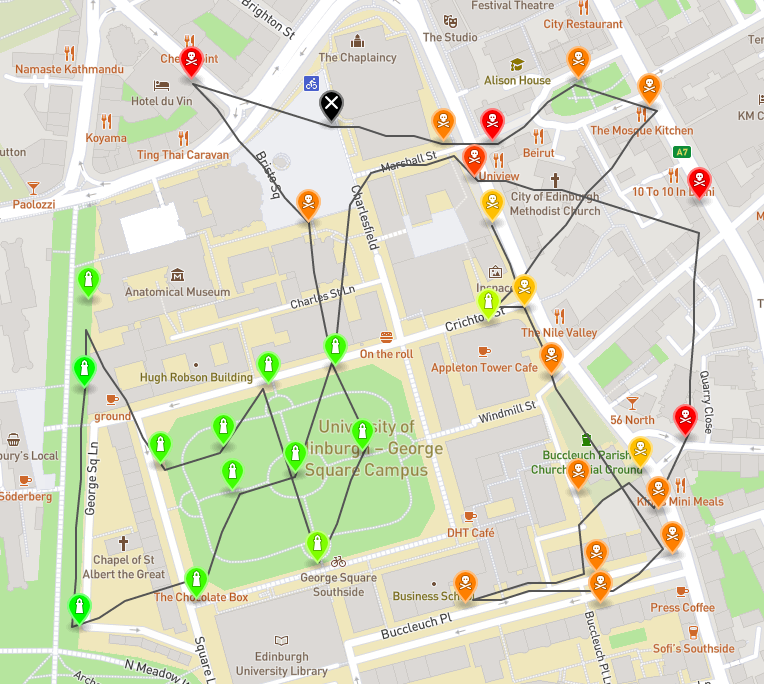
\includegraphics[width=0.75\textwidth]{01-01-2020}
\end{center}

The second picture is from a drone run on \textbf{05/05/2020}, starting again from the same location $(55.944425, -3.188396)$. The screenshow is below:

\begin{center}
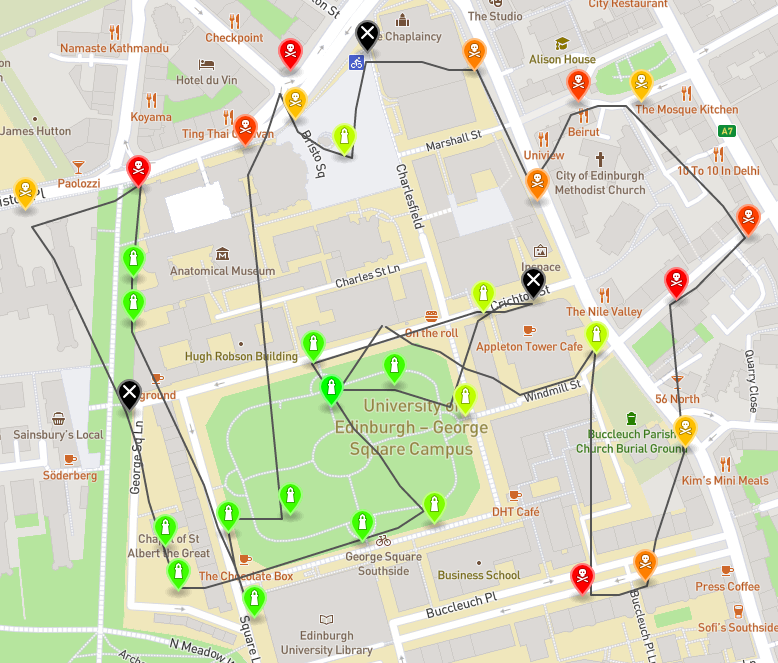
\includegraphics[width=0.75\textwidth]{05-05-2020}
\end{center}



%%%%%%%%%%%%%%%%%%%%%%%%%%%%%%%%%%%%%%%%%%%%%%%%%%%%%%%%%%%%%%%%%%%%%%%%%%%%%%%%%%%%%%%%

\addcontentsline{toc}{section}{References}
\bibliography{sources} 
\bibliographystyle{ieeetr}

\end{document}